\documentclass[a4paper]{article}

%% Language and font encodings
\usepackage[english]{babel}
\usepackage[utf8x]{inputenc}
\usepackage[T1]{fontenc}
\usepackage{bbold}

%% Sets page size and margins
\usepackage[a4paper,top=3cm,bottom=2cm,left=3cm,right=3cm,marginparwidth=1.75cm]{geometry}

%% Useful packages
\usepackage{amsmath}
\usepackage{graphicx}
\usepackage[colorinlistoftodos]{todonotes}
\usepackage[colorlinks=true, allcolors=blue]{hyperref}

\title{Trabalho Computacional 2 - Resolução Numérica de Equações Diferenciais
usando Elementos Finitos}
\author{Luiz Guilherme de Carvalho Lopes}

\begin{document}
\maketitle

\maketitle

\section{Introdução}



As equações diferenciais no mundo contemporâneo têm papel fundamental. Ser capaz de descrever matematicamente o comportamento de fluidos, como por exemplo o arrasto causado por um fluido passando por uma placa plana, através da equação diferencial de Navier-Stokes, entre diversas outras coisas, permitiram ao homem o advento do avião. Portanto compreender e aplicar o método de elementos finitos para a resolução de E.D.O. que não podem ser resolvidas algebricamente é essencial.

\section{questão 1}

\ \ \ \  Muitas vezes nas equações diferencias achar o resultado exato é algo impossivel, por isso optamos por encontrar uma outra função que mesmo não sendo o resultado exato, esta função seja o mais próxima possível do resultado exato, com isto o método de elementos finitos é uma ferramenta capaz de encontrar uma função que esteja o mais próximo possível da resposta correta.

A ideia do método é discretizar o domínio do problema e em vez de encontrar uma solução da equação para todo o domínio, encontramos uma solução para alguns pontos do domínio, e quanto maior o número de pontos considerados, melhor será nossa solução, tendo isso em vista sempre haverá um erro associado a esta resolução, pois se fosse possível encontrar a solução para todos os pontos do domínio seria necessario discretizar todos os infinitos pontos, o que é impossível já que o computador é uma maquina finita.

Considere o problema de equação diferencial:
\(-u''(x)=f(x)\) com valores de contorno  \(u(0)=u(1)=0 \).


O primeiro passo a ser dado é considerar o espaço vetorial \(H_{0}^{1}\)=(\(g\in C^{\infty} [0,1] :|g|<{\infty}, g(0)=g(1)=0 \)), note que a função a ser encontrada é tal que ela pertence ao espaço \(H_{0}^{1}\) e também considere como produto interno de funções \(<g,h>= \int_{0}^{1}g(x)h(x)dx \).

A equação inicial pode ser reformulada da seguinte maneira: \(-u''(x)=f(x)\) 

\(-u''(x)-f(x)=0\)

\(\int_{0}^{1}(-u''(x)-f(x))v(x)dx=0\),  \(\forall v,u\in H_{0}^{1} \)

\(\int_{0}^{1}-u''(x)v(x)dx\) -\(\int_{0}^{1}f(x)v(x)dx\)=0 fazendo integral por partes na primeira integral ficamos com:

\(-u'(x)v(x)|_{0}^{1}\)\(+\int_{0}^{1}u'(x)v'(x)dx-\int_{0}^{1}f(x)v(x)dx=0\) ao aplicar os limites de integração ficamos com:

\(\int_{0}^{1}u'(x)v'(x)dx=\int_{0}^{1}f(x)v(x)dx\),   \(\forall u,v\in H_{0}^{1} \)

Agora com esta equação iremos aplicar a discretização.

\subsection{Discretização}

Vamos considerar as funções \(V \in H_{0}^{1} \), chamadas de funções HAT.Estas funções serão responsáveis por cobrir todo o domínio do nosso problema, na qual em um parte do domínio  ela ira variar de forma linear ate atingir o valor de pico, sendo esse valor 1, e depois decrescendo de forma linear ate atingir o valor zero novamente, e no resto do domínio terá valor zero.

\clearpage

\begin{figure}
\centering
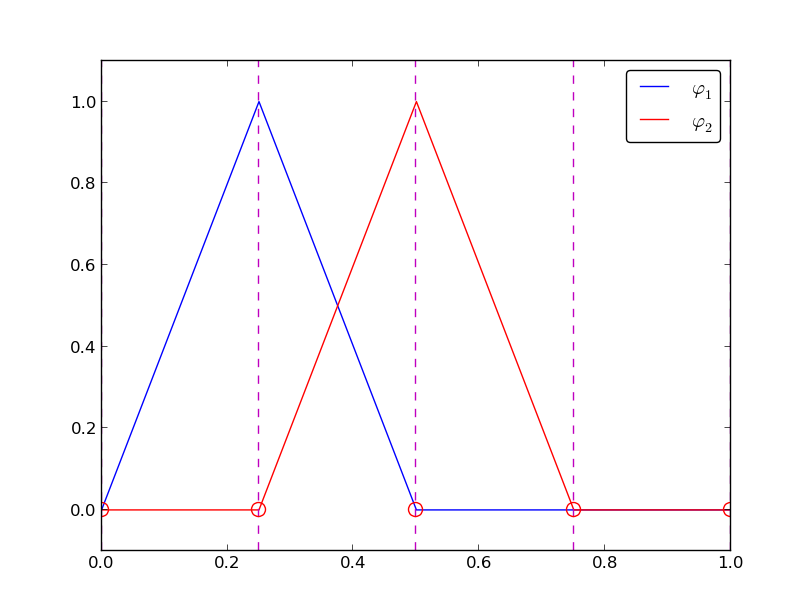
\includegraphics[width=0.53\textwidth]{hat_functions.png}

\caption{exemplo de discretização do domínio[0,0.8] com duas funções HAT.}
\end{figure}



 Este é um exemplo de um domínio coberto por 2 funções HAT, note que nesse caso o domínio seria o intervalo [0, 0.8], no nosso caso seria necessário uma terceira função HAT para cobrir toda o domínio. No entanto apenas 3 funções HAT para cobrir o nosso domínio seria uma aproximação insuficiente para se obter um resultado adequado, portanto quanto maior o numero de funções HAT melhor será nossa aproximação, no entanto o número de dados a ser tratado pelo computador também aumenta fazendo necessário uma escolha boa para o número de funções HAT.
 
 Observe que na figura dividindo o domínio em 4 partes foi necessário 3 funções HAT para cobri-lo, com isto se fizermos n divisões no domínio, teremos n-1 funções HAT, com isto  \(n\in \mathbb{N}\) é o número de partes que dividiremos o nosso domínio.
 
 Agora considere o subespaço vetorial \(S_{n}\)=SPAN\((V_1,...,V_{n-1})\), \(g=c_1V_1+...+c_{n-1}V_{n-1}\), onde \(c_i \in \mathbb{N},  \forall i \in ({1, \dots ,n-1}) \).A combinação linear desses vetores é que vai gerar nossa solução aproximada da função \(u(x)\), e veja que o método é implementado para os valores no contorno terem seus valores exatos.
 
 Agora o nosso problema se transformou em descobrir os valores dos coeficientes \(c_i\) uma vez encontrados teremos nossa solução aproximada.Veja que a equação anterior ainda depende de descobrimos a equação de cada uma das funções HAT para cada n escolhido, o embasamento teórico para a determinação da função HAT assim  como de suas derivadas, que serão necessárias para a resolução do problema, será feito sem mostrar todos os passos, aqui será entendido que o leitor já tem o conhecimento básico de como encontrar a equação de curvas simples.
 
\[V_i=
\left \{
  \begin{tabular}{cc}
 \ \ \(n(x-(\frac{i-1}{n}))\)& ,\(\forall x \in [\frac{i-1}{n},\frac{i}{n}]\)  \\
  \(-n(x-(\frac{i+1}{n}))\) & ,\(\forall x \in (\frac{i}{n}, \frac{i+1}{n}]\) \\
  0 &, se x \(\not\in [\frac{i-1}{n},\frac{i+1}{n}] \)
  \end{tabular}
\right \}
\]  
\[V'_i=
\left \{
  \begin{tabular}{cc}
  \ \ n & ,\(\forall x \in (\frac{i-1}{n},\frac{i}{n})\)  \\
  \ -n & ,\(\forall x \in (\frac{i}{n}, \frac{i+1}{n})\) \\
 \ \ 0 &, se x \(\not\in [\frac{i-1}{n},\frac{i+1}{n}] \)
  \end{tabular}
\right \}
\] 

\[V'_iV'_i=
\left \{
  \begin{tabular}{cc}
  \(n^{2}\) & ,\(\forall x \in (\frac{i-1}{n},\frac{i}{n})\)  \\
  \(n^{2}\) & ,\(\forall x \in (\frac{i}{n}, \frac{i+1}{n})\) \\
  0 &, se x \(\not\in [\frac{i-1}{n},\frac{i+1}{n}] \)
  \end{tabular}
\right \}
\] 
\(\forall i \in (1,...,n-1)\)
\[V'_iV'_{i+1}=
\left \{
  \begin{tabular}{cc}
  0 & ,\(\forall x \not\in (\frac{i-1}{n},\frac{i}{n})\)  \\
  \(-n^{2}\) & ,\(\forall x \in (\frac{i}{n}, \frac{i+1}{n})\) 
  \end{tabular}
\right \}
\] \(\forall i \in (1,...,n-2)\)

\(V'_iV'_k=0,\) se \(|i-k|>1,\forall i,k \in (1,...,n-1)\)

Finalmente voltando para a equação:\(\int_{0}^{1}u'(x)v'(x)dx=\int_{0}^{1}f(x)v(x)dx\),   \(\forall u,v\in H_{0}^{1} \) temos que ela é válida para cada \(V_i\) e também vamos reescrever \(u(x)\) como uma combinação linear de \(V_i\)

\(\int_{0}^{1}(c_1V_1+...+c_{n-1}V_{n-1})V'_i(x)dx\)=\(\int_{0}^{1}f(x)V_i(x)dx\), \(\forall i \in (1,...,n-1)\) 

\(c_1 \int_{0}^{1}V'_1 V'_idx+ ... + c_{n-1}\int_{0}^{1}V'_{n-1}V'_idx\)=\(\int_{0}^{1}f(x)V_idx\), fazendo todas as equações ficamos com:

\((\int_{0}^{1}V'_1V'_1dx)c_1+...+(\int_{0}^{1}V'_{n-1}V'_1dx)c_{n-1}\)=\(\int_{0}^{1}f(x)V_1dx\) 

\ \ \ \ \ \ \ \ \ \ \ \ \ \ \ \ \ \ \ \ \ \ \ \ \ \ \ \ \ \ \ \ \ \ \ \ \ \   \vdots
 
 \((\int_{0}^{1}V'_1V'_{n-1}dx)c_1+...+(\int_{0}^{1}V'_{n-1}V'_{n-1}dx)c_{n-1}\)=\(\int_{0}^{1}f(x)V_{n-1}dx\) 
 
 todas essas equações podem ser reescritas na forma de uma equação matricial.
 
 \( \begin{bmatrix}
  \int_{0}^{1}V'_1V'_1dx &  \dots &  \int_{0}^{1}V'_{n-1}V'_{1} \\
   \vdots & \ddots & \vdots \\
   \int_{0}^{1}V'_1V'_{n-1}dx & \dots & \int_{0}^{1}V'_{n-1}V'_{n-1}\\
   \end{bmatrix}\) \(\begin{bmatrix}
   c_1 \\
   \vdots \\
   c_{n-1}
   \end{bmatrix}\)=\(\begin{bmatrix}
   \int_{0}^{1}f(x)V_1dx \\
   \vdots \\
   \int_{0}^{1}f(x)V_{n-1}dx \\
   \end{bmatrix}\)
   
   Agora resolvendo as integrais temos: \(\int_{0}^{1}V'_iV'_idx\)=\(\int_{\frac{i-1}{n}}^{\frac{i+1}{n}}n^{2}dx\)=\(n^{2}(\frac{2}{n})\)=2n \\
  \(\int_{0}^{1}V'_iV'_{n+1}dx\)=\(\int_{\frac{i}{n}}^{\frac{i+1}{n}}-n^{2}dx\)=\(-n^{2}(\frac{1}{n})\)=-n , e caso \(|i-k|>1\),para \(i,k\in (1,...,n-1)\) \(\int_{0}^{1}V'_iV'_kdx=0\) \\
  
 Com isto obtemos: \(\begin{bmatrix}
 2n & -n & 0 & \dots & 0 & 0 & 0  \\
 -n & 2n & -n & 0 & \dots & 0 & 0 \\
 0 & -n & 2n & -n & 0 & \dots & \vdots \\
 \vdots & \vdots & \ddots & \ddots & \ddots & \vdots & -n \\
 0 & 0 & 0 & 0 & \dots & -n & 2n \\
 \end{bmatrix}\)\(\begin{bmatrix}
 c_1 \\
 c_2 \\
 c_3 \\
 \vdots \\
 c_{n-1} \\
 \end{bmatrix}\)=\(\begin{bmatrix}
 \int_{0}^{1}f(x)V_1dx \\
 \int_{0}^{1}f(x)V_2dx \\
 \int_{0}^{1}f(x)V_3dx \\
 \vdots \\
 \int_{0}^{1}f(x)V_{n-1}dx \\
 \end{bmatrix}\).
 
 
 
 Esta equação matricial e da forma Ax=B, com  \(A=\begin{bmatrix}
 2n & -n & 0 & \dots & 0 & 0 & 0  \\
 -n & 2n & -n & 0 & \dots & 0 & 0 \\
 0 & -n & 2n & -n & 0 & \dots & \vdots \\
 \vdots & \vdots & \ddots & \ddots & \ddots & \vdots & -n \\
 0 & 0 & 0 & 0 & \dots & -n & 2n \\
 \end{bmatrix}\),
 
 \(B=\begin{bmatrix}
 \int_{0}^{1}f(x)V_1dx \\
 \int_{0}^{1}f(x)V_2dx \\
 \int_{0}^{1}f(x)V_3dx \\
 \vdots \\
 \int_{0}^{1}f(x)V_{n-1}dx \\
 \end{bmatrix}\) e \(x=\begin{bmatrix}
 c_1 \\
 c_2 \\
 c_3 \\
 \vdots \\
 c_{n-1} \\
 \end{bmatrix}\) \(A \in M(n-1 \times n-1), B \in M(n-1 \times 1)\) e \(x \in M(n-1 \times 1)\)
 
 
 
 
 A primeira matriz é conhecida como a matriz tridiagonal, na qual há uma quantidade significativa de zeros, que permite o sistema linear \(Ax=b\) seja resolvido de maneira efetiva.
 
 Com o sistema resolvido encontramos os coeficientes \(c_1,\dots, c_{n-1}\) e com isto encontramos \(u(x)=(c_1V_1+ \dots + c_{n_1}V_{n_1})\) como nossa solução aproximada, veja que ainda é necessário encontrarmos os valores da matriz B. 
 
 O algortimo utilizado para montar a matriz A do sistema linear em linguagem de matlab esta escrito abaixo.
  
  A=zeros(n-1,n-1) ;
  
  for k=1:n-1 ;
  
  A(k,k)=2*n ;
  
  end
  
  for k=1:n-2 ;
  
  A(k+1,k)=-1*n ;
  
  A(k,k+1)=-1*n ;
  
  end 
  
  
  

  \section{questão 2}
  
  Com a função \(f(x)=-x^3+5\) conseguimos encontrar os valores das entradas da matriz B.
  
  Temos que resolver a integral \(\int_{0}^{1}f(x)V_idx, \forall i \in (1,\dots, n-1)\) esta resolução é demasiadamente longa e no contexto deste trabalho fica entendido que o leitor tem condições de resolver esta integral, com isto \(\int_{0}^{1}f(x)V_idx=-\frac{i^3}{n^4}-\frac{i}{2^4}+\frac{5}{n}\), \(\forall i \in (1,\dots, n-1)\).
  Agora podemos montrar a matriz B em linguagem de matlab, o algoritmo utilizado esta escrito abaixo.
  
  for k=1:n-1 ;
  
  B(k,1)=\((-k\string^3/n\string^4)-k/(2*(n\string^4))+(5/n)\) ;
  
  end

  O algoritmo utilizado para a montagem do sistema será enviado via e-mail, definida a densidade da malha(o valor de n) e com o algoritmo de montagem feito, podemos determinar as matrizes A e B do sistema linear. Com todas estas informações em mãos podemos utilizar o matlab para resolver o sistema linear usando o comando $x=A \backslash B$. Depois disto foi desejado que a matriz x fosse tal que os valores extremos dela sejam zeros, devido ao fato dos valores de contorno serem zero também, com isto usamos o comando em matlab \(x=\begin{bmatrix}
  0 & x' & 0 \\
  \end{bmatrix}\).
  
  
  
Com a matriz x temos o valor exato da função em n+1 pontos, como as funções \(V_i\) são retas, temos que a combinação linear destas funções também serão retas, e portanto tendo os pontos exatos precisamos ''liga-los'' atraves de retas e com isto teremos nossa solução aproximada.

O algoritmo utilizado para encontrar a solução aproximada também será enviada por e-mail, no entanto há alguns pontos que gostaria de enfatizar, e portanto colocarei o algoritmo abaixo, em linguagem de matlab.

function\([V]\)= solucao$\_$aproximada(k,n,x)

      for i=1:n;
          
          for j=1: \(\frac{(k-1)}{n}\);

          \(V(j+((k-1)/n)*(i-1))= x(i) + n*(x(i+1)-x(i))*(j-1)/(k-1)\);

          end

      end
   
     \(V(k)=0;\)
     
     Da forma que o algoritmo foi montado há duas considerações a serem feitas:
     
     1) o valor k que aparece no algoritmo é o número total de pontos que a solução aproximada terá, incluindo os pontos extremos, como o computador é uma máquina finita precisamos estipular um bom valor de k para compararmos a solução exata da solução aproximada, e com isto temos as seguintes questões: o que seria um bom valor de k? quando k é grande o suficiente para termos uma aproximação confiável? estes questionamento são relevantes e podem ser explorados em um proximo trabalho, e neste trabalho foi estipulado que k=20001 é um valor suficientemente grande para a solução ser confiável, estas mesmas considerações também são validas para o valor de n.

    2) perceba que a divisão \(\frac{(k-1)}{n}\) obrigatoriamente tem que ser um número natural, caso contrário o algoritmo não fara sentido, ou seja, k-1 tem q ser múltiplo de n.
    
    \subsection{explicação do algoritmo}

   O vetor x possui n-1 pontos com o valor exato, e também mais 2 pontos(os pontos extremos) com o valor exato, mas deseja-se completar os pontos intermediários de tal forma que hajá uma quantidade significativa de pontos, como os pontos determinados pelo vetor x serão interligados atraves de retas, o algoritmo completa o vetor x com os pontos intermedíarios chegando no vetor \(V\) que é a solução aproximada com k pontos.

Para entender o algoritmo é necessário o conhecimento básico de geometria analítica e de equações polinomiais de primeiro grau.

Deseja-se que no total tenha uma quantidade de k pontos, sendo que destes k pontos, n+1 pontos são exatos, seja q a quantidade de pontos a serem completados entre 2 pontos exatos, como há n+1 pontos exatos haverá n intervalos para serem completados por q pontos, então no total teremos \((n+1)+n.q=k\), disto concluimos que \(q=\frac{k-1}{n}-1\).

Agora precisamos do coeficiente angular de cada um das n retas a serem formadas, sendo m o coeficiente angular da reta temos \(m=\frac{x(i+1)-x(i)}{\frac{1}{n}}=n(x(i+1)-x(i)), \forall i \in (1,...,n) \). Com o coeficiente angular podemos determinar o valor de cada ponto, sabemos que o valor de cada ponto entre \(x(i)\) e \(x(i+1)\) será o valor \(x(i)\) com um acréscimo dada pelo coeficiente angular \(m\) dada uma variação no domínio \(\Delta x \), assim como havera \(q\) pontos que divide cada intervalo de tamanho \(\frac{1}{n}\) teremos este intervalo subdividido em \(q+1\) intervalos, ou seja, teremos \(\frac{k-1}{n}\) subintervalos, cada subintervalo terá o tamanho de \(\frac{\frac{1}{n}}{\frac{k-1}{n}}=\frac{1}{k-1}\), mas para cada ponto teremos \(\Delta x=\frac{1}{k-1}\) multiplicado por um valor \((j-1) \in \mathbb{N} \) sendo \(j\) um valor que varia de 1 até \(q+1=\frac{k-1}{n}\), aqui precisamos que \((j-1)\) tenho valor zero para considerarmos o ponto \(x(i)\) dentro do vetor \(V\). Da parte do algoritmo  \(V(j+((k-1)/n)*(i-1))\) com \(j\) variando de 1 até \(\frac{k-1}{n}\)  e i fixo igual a 1, teremos apenas a primeira reta formada, precisamos que i varia de 1 até n, mas veja que quando j atinge o ultimo valor em \(\frac{k-1}{n}\) temos que a cada variação de i precisamos que este valor seja multiplicado por \(\frac{k-1}{n}\), para que \(V\) seja montado de forma correta, e também precisamos que a última entrada do vetor \(V\) seja 0. Com isto teremos o nosso vetor \(V\) formado.
  
  \clearpage
  
  
  Utilizando a função diags montamos a matriz A da seguinte forma em linguagem de matlab:
  
  S=2*n*ones(1,n-1) ;
  
  D=-1*n*ones(1,n-2); 
  
  A=diag(S)+diag(D,-1)+diag(D,1) ;
  
  podemos utilizar estes comando para formar a matriz A em vez de utilizarmos o algoritmo montegem\_sistema.
  
  \section{questão 3}
  
  Utilizando os algoritmos descritos acima foi montado a solução exata em linguagem de matlab da seguinte forma:
  
  E=[0:\(\frac{1}{(k-1)}:1\)];
  
  f=\((E.\string^5)/20 +(-5*E.\string^2)/2 +(49*E)/20\) % corrigir essa coisa 
  
  Observe que a solução exata também foi dividida em k pontos.
  
  Para computar o maior erro entre a solução exata e a aproximada e a construção do gráfico foi utilizado os seguintes codigos em linguagem de matlab:

  \(norm(V-f,'inf')\)

  \(plot(E,f);\)

   hold on;

  \(plot(E,V,'r')\)

Para o erro ser inferior a \(10^{-4}\), foi necessário que o valor de n fosse superior a 80, para o erro ser inferior a \(10^{-6}\), foi necessário que o valor de n fosse superior a 800 e para o erro ser inferior a \(10^{-8}\), foi necessário que o valor de n fosse superior a 10000. \\ 

\begin{figure}[h]
\begin{minipage}[t][5cm][b]{0,5\textwidth} 
  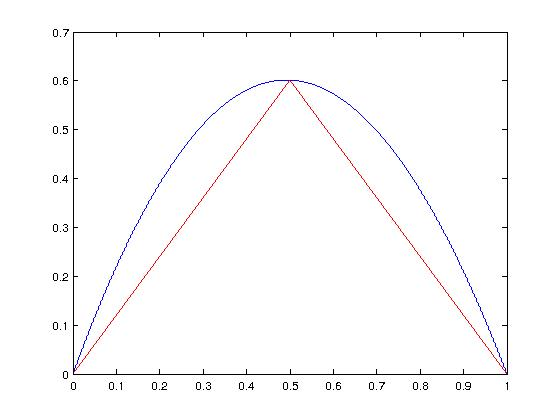
\includegraphics[width=\textwidth]{n_2__0_1555.jpg} 
  \end{minipage}
  \begin{minipage}[t][5cm][b]{0,5\textwidth}
  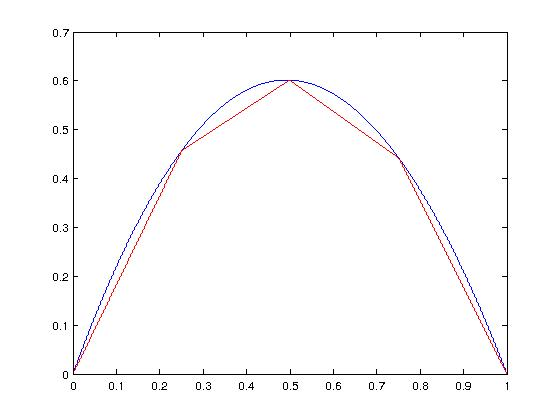
\includegraphics[width=\textwidth]{n_4__0_0390.jpg}
  \end{minipage} 
  \begin{minipage}[t][5cm][b]{0,5\textwidth}
  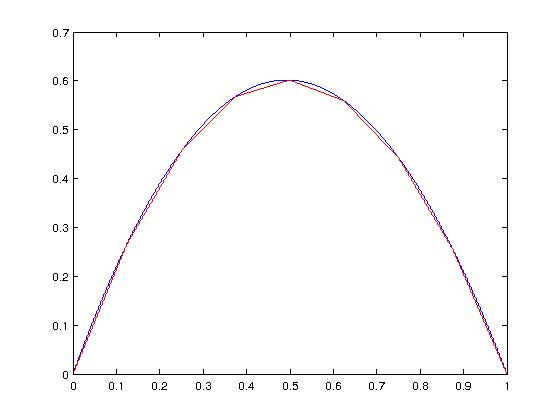
\includegraphics[width=\textwidth]{n_8__0_0098.jpg}
  \end{minipage} 
  \begin{minipage}[t][5cm][b]{0,5\textwidth}
  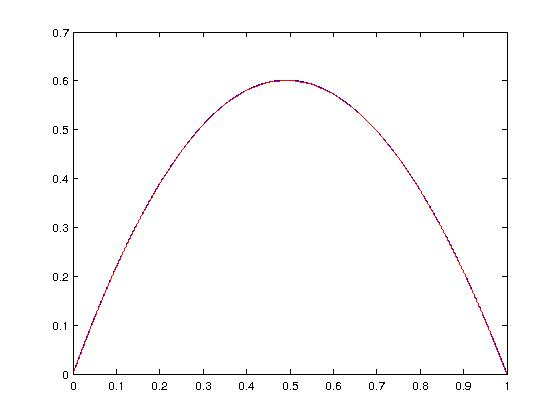
\includegraphics[width=\textwidth]{n_20__0_0016.jpg}
  \end{minipage}
  \caption{figura do topo da esquerda: solução aproximada com \(n=2\) e erro máximo igual a 0.1555.}
  \caption{figura do topo da direita: solução aproximada com \(n=4\) e erro máximo igual a 0.039.}
\caption{figura de baixo da esquerda: solução aproximada com \(n=8\) e erro máximo igual a 0.0098.}
\caption{figura de baixo da direita: solução aproximada com \(n=20\) e erro máximo igual a 0.0016.}
  \end{figure}
  
  \clearpage
  
   Em azul temos a solução exata, e em vermelho a solução aproximada,observe que com uma quantidade superior a 20 para a densidade da malha(valor de n), teremos que a diferença entre a solução exata e a solução aproximada já não é mais visível a olho nu.
  
  
  
  
  \section{questão 4}
  
  Agora iremos utilizar o comando esparse do matlab para montar o sistema linear Ax=B, com esse comando conseguimos construir as matrizes do problema sem que o computador considere as entradas nulas, evitando um gasto de memória desnecessário e otimizando o processo, permitindo resolver problemas de grande porte.
  
  Para montarmos a matriz tridiagonal A, utilizaremos o comando esparse da seguinte forma.

I=[1:n-1];

val=2*n*ones(1,n-1);

P=sparse(I,I,val);

Q=[2:n-1];

W=[1:n-2];

L=-1*n*ones(1,n-2);

O=sparse(Q,W,L,n-1,n-1);

K=sparse(W,Q,L,n-1,n-1);

A=P+O+K

Com isto montamos nossa matriz A com menor quantidade de informação, e utilizando o comando $x=A \backslash B$ conseguimos resolver o sistema linear de forma otimizada.

Anteriormente utilizando o comando diag para montar o sistema linear, conseguiamos resolver o problema quando o valor de n fosse inferior ou igual a 10000, com este valor para n o computador utilizado demorava cerca de 12 segundos.

Utilizando as matrizes esparsas conseguimos resolver o problema em menor tempo e também utilizando um valor maior para a densidade da malha, desta forma fomos capazes de utilizar o valor de k=5120001, e o valor de n=640000, resolvendo o problema em 3 segundos e com o maior erro sendo  \(1.0232.10^{-09}\), e com k=10240001 e n=2560000 ainda fomos capazes de resolver o problema, no entanto para valores superiores a este o computador por vezes travava e não conseguia resolver o problema.


  
  \begin{table}[h]
\centering
\caption{tabela comparativa do tempo computacional utilizando a função diag(matriz densa) e utilizando o comando sparse.}
\label{my-label}
\begin{tabular}{|l|l|l|l|l|l|l|l|}
\hline
densidade da malha  & 10       & 50       & 100      & 500      & 2000     & 5000     & 10000     \\ \hline
diag (em segundos)  & 0.092142 & 0.087258 & 0.082371 & 0.082601 & 0.285727 & 2.031926 & 12.599604 \\ \hline
sparsa (em segundos) & 0.076553 & 0.078695 & 0.080297 & 0.078371 & 0.079250 & 0.085030 & 0.095693  \\ \hline
\end{tabular}
\end{table}

\section{Bibliografia}

Gilbert Strang. Linear Algebra and its Aplication. Quarta edição. Editora Thomson.
   
  
  

 
  
   

\end{document}